\documentclass[12pt,a4paper]{article}
\usepackage{amsmath}
\usepackage[english]{babel}
\usepackage{graphicx}
\usepackage{listings}
\usepackage{fullpage}
\usepackage[T1]{fontenc}

\lstdefinestyle{custompython}{
  belowcaptionskip=1\baselineskip,
  breaklines=true,
  frame=L,
  xleftmargin=\parindent,
  language=bash,
  basicstyle=\footnotesize\ttfamily,
  showstringspaces=false,
  %commentstyle=\itshape\color{purple!40!black},
  %keywordstyle=\itshape\color{green!40!black},
  %identifierstyle=\color{blue},
  %stringstyle=\color{orange},
}

\author{
  Cheng, Lidens\\
  \texttt{lidenscheng@email.arizona.edu}
  \and
  McClintock, Tom\\
  \texttt{tmcclintock@email.arizona.edu}
  \and
  Wagoner, Erika\\
  \texttt{wagoner47@email.arizona.edu}
}
\title{Astr 513: Homework 1}

\begin{document}
\maketitle
  
\section{Random Number Generators}

\section{Designing surveys}

\section{Blackbody Distribution}
\subsection{}
Given our initial distribution:
\begin{equation*}
  f(\epsilon;T)d\epsilon = C\frac{\epsilon^2d\epsilon}{\exp{(\epsilon/kT)}-1}
\end{equation*}
we first make a change in variables $\epsilon' = \epsilon/kT$. This results
in the distribution
\begin{equation*}
  f(\epsilon')d\epsilon' = A\frac{\epsilon'^2d\epsilon'}{\exp{(\epsilon')}-1}
\end{equation*}
where $A=C(kT)^2$.
\subsection{}
We now need to find where this function is a maximum numerically. First we
define our function in Python:
\begin{lstlisting}[style=custompython]
  def f(eps):
      return eps**2/(np.exp(eps)-1)
\end{lstlisting}
and find its maximum. This was found to be at the 
location $\epsilon'\approx1.594$.
\subsection{}
We now renormalize by dividing by $f(\epsilon=1.594)\approx0.6476$.
This yields:
\begin{equation*}
  f'(\epsilon')d\epsilon' = B\frac{\epsilon'^2d\epsilon'}{\exp{(\epsilon')}-1}
\end{equation*}
where $B=A/0.6476$.
\subsection{}
We define a function to return a photon of energy between $\epsilon'_1=0.1$
and $\epsilon'_2=5.0$.
\begin{lstlisting}[style=custompython]
  def en(eps):
      return np.random.rand()*(5.0-0.1)+0.1
\end{lstlisting}
\subsection{}
We now make repeated draws to this function to get a collection of $N$
photon energies ${e_i},\ i\in[1,N]$. Additionally, we draw $N$ random
numbers between $0$ and $1$, ${r_i},\ i\in[1,N]$. If $f'(\epsilon'_i) < r_i$
then the photon is removed from the list. We do this for $N=100000$.
\subsection
Histogramming the photons yields a version of the distribution
with the area of the bins normalized to $1$.
\begin{figure*}[!h]
  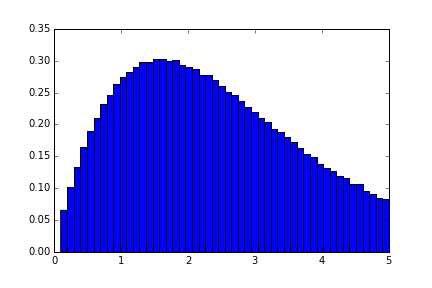
\includegraphics[]{HW1_3_6_normalized.png}
\end{figure*}
If we simply loop over the energy domain and plot the fraction of accepted
photons in that bin then we recover $f'$.
\begin{figure*}[!h]
  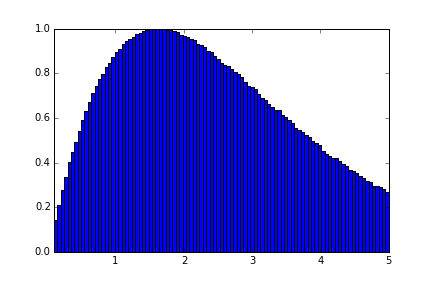
\includegraphics[]{HW1_3_6.png}
\end{figure*}

\end{document}
